\newpage
\subsection{Visual; emptying}
\visHeader
\hypertarget{emptyPartition vis}{}

To create a \emph{for each} story node, create the initial diagram and start node for the method \texttt{Partition::empty}, then \emph{quick create} an 
activity node choosing \texttt{ForEach} as its type (Fig.~\ref{fig:sdm_foreach}).

\begin{figure}[htbp]
\begin{center}
  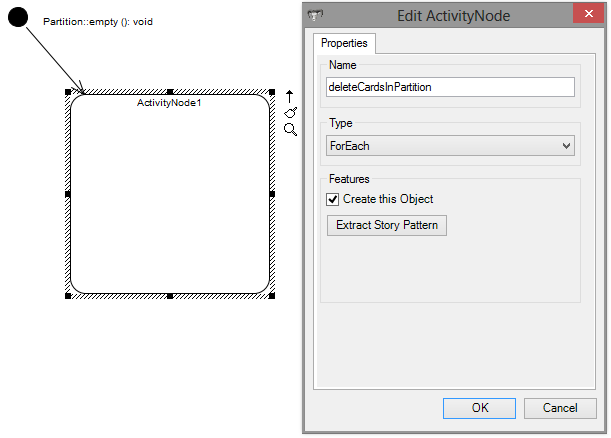
\includegraphics[width=0.9\textwidth]{ea_forEach}
  \caption{A for each loop in SDM.}  
  \label{fig:sdm_foreach}
\end{center}
\end{figure}

A \emph{for each} story node is visualised as a double node to indicate potential repetition.  Complete the story pattern as indicated in
Fig.~\ref{fig:sdm_end}.   Please note that the \texttt{card} that is deleted in each match is unbound, and both the \texttt{card} and link to \texttt{this} are
set to \texttt{destroy}. Even more important, note that the guard that terminates the for each story node has an \texttt{[end]} guard. Indeed, a \emph{for% 
each} story node \emph{must} have an end activity edge which is taken when all matches for the story pattern have been handled.

There are two interesting points to note: First of all, how would the pattern be interpreted if the story node was a normal story node, not a \emph{for each}?
Well, the pattern would specify that \emph{a} card should be matched and deleted from the current partition, and that's it. Note that the \emph{exact} card is
not specified and indeed the actual choice of the card is \emph{non-deterministic} or random.  This is a common property of graph transformations and pattern
matching, and is something that takes some to get used to.  In general, there are no guarantees concerning the choice and order of valid matches.

\begin{figure}[htbp]
\begin{center}
  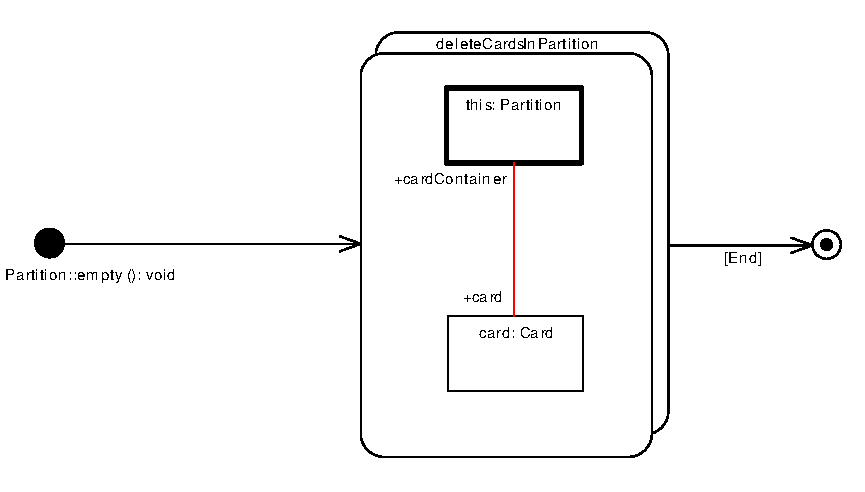
\includegraphics[width=0.9\textwidth]{ea_completeActivityEmptyCards.pdf}
  \caption{Complete story pattern with \texttt{[end]} guard.}  
  \label{fig:sdm_end}
\end{center}
\end{figure}

A second point is deciding if we need to destroy the link between \texttt{this} and \texttt{card}. Would the pattern be interpreted differently if we just destroyed
\texttt{card} and left the link?  The answer is no, the pattern would yield the same result, regardless of if the link is explicitly destroyed or not.
This is because the transformation engine we use\footnote{CodeGen2 which is part of Fujaba \url{http://www.fujaba.de/}} ensures that there are never any
\note{Dangling Edges} \emph{dangling edges} in a model.  As deleting only \texttt{card} would result in a ``dangling edge'' attached to \texttt{this}, the link
is deleted as well. Explicitly destroying the link is therefore a matter of taste, but \ldots why not be as explicit as possible?
